\documentclass[problem]{mcs}

\begin{pcomments}
  \pcomment{from: S09.cp2m}
  \pcomment{skipped in S09 (maybe commented out because it doesn't appear in .pdf)}
\end{pcomments}

\pkeywords{
  binary
  logic
  circuits
  boolean
}

%%%%%%%%%%%%%%%%%%%%%%%%%%%%%%%%%%%%%%%%%%%%%%%%%%%%%%%%%%%%%%%%%%%%%
% Problem starts here
%%%%%%%%%%%%%%%%%%%%%%%%%%%%%%%%%%%%%%%%%%%%%%%%%%%%%%%%%%%%%%%%%%%%%

\begin{problem}
Considerably faster adder circuits work by computing the values in later
columns for both a carry of 0 and a carry of 1, \emph{in parallel}.  Then,
when the carry from the earlier columns finally arrives, the pre-computed
answer can be quickly selected.  We'll illustrate this idea by working out
the equations for an $n+1$-bit parallel half-adder.

Parallel half-adders are built out of parallel ``add1'' modules.  An
$n+1$-bit add1 module takes as input the $n+1$-bit binary representation,
$a_n \dots a_1 a_0$, of an integer, $s$, and produces as output the binary
representation, $c\,p_n\dots p_1\,p_0$, of $s+1$.

\bparts

\ppart A 1-bit add1 module just has input $a_0$.  Write propositional
formulas for its outputs $c$ and $p_0$.

\begin{solution}
\begin{align}
p_0 & = a_0\ \QXOR\ 1 = \QNOT(a_0)\\
c & = a_0.
\end{align}
\end{solution}

\ppart Explain how to build an $n+1$-bit parallel half-adder from an
$n+1$-bit add1 module by writing a propositional formula for the
half-adder output, $o_i$, using only the variables $a_i$, $p_i$, and $b$.

\begin{solution}
\[
o_i  = (b\ \QAND\ p_i)\ \QOR\ (\QNOT(b)\ \QAND\ a_i)
\]
\end{solution}

\eparts

We can build a double-size add1 module with $2(n+1)$ inputs using two
single-size add1 modules with $n+1$ inputs.  Suppose the inputs of the
double-size module are $a_{2n+1},\dots, a_1, a_0$ and the outputs are
$c,p_{2n+1},\dots, p_1,p_0$.  The setup is illustrated in
Figure~\ref{fig:add1}.

Namely, the first single size add1 module handles the first $n+1$ inputs.
The inputs to this module are the low-order $n+1$ input bits $a_n,\dots,
a_1, a_0$, and its outputs will serve as the first $n+1$ outputs $p_n,
\dots, p_1, p_0$ of the double-size module.  Let $c_{(1)}$ be the
remaining carry output from this module.

The inputs to the second single-size module are the higher-order $n+1$
input bits $a_{2n+1}, \dots, a_{n+2}, a_{n+1}$.  Call its first $n+1$
outputs $r_n, \dots, r_1, r_0$ and let $c_{(2)}$ be its carry.

\bparts

\ppart Write a formula for the carry, $c$, in terms of $c_{(1)}$ and
$c_{(2)}$.

\begin{solution}
\[
c = c_{(1)}\ \QAND\ c_{(2)}.
\]
\end{solution}

\ppart Complete the specification of the double-size module by writing
propositional formulas for the remaining outputs, $p_i$, for $n+1 \leq i
\leq 2n+1$.  The formula for $p_i$ should only involve the variables
$a_i$, $r_{i-(n+1)}$, and $c_{(1)}$.

\begin{solution}
  The $n+1$ high-order outputs of the double-size module are the
  same as the inputs if there is no carry from the low-order $n+1$
  outputs, and otherwise is the same as the outputs of the second
  single-size add1 module.  So
\begin{equation}\label{parallel-pi}
p_i = (\QNOT(c_{(1)})\ \QAND\ a_i)\ \QOR\ (c_{(1)}\ \QAND\ r_{i-(n+1)}).
\end{equation}
for $n+1 \leq i \leq 2n+1$.
\end{solution}

\ppart Parallel half-adders are exponentially faster than ripple-carry
half-adders.  Confirm this by determining the largest number of
propositional operations required to compute any one output bit of an
$n$-bit add module.  (You may assume $n$ is a power of 2.)

\begin{solution} 
  The most operations for an output are those specified in
  formula~\eqref{parallel-pi}.  So it takes at most 4 additional
  operations to get any one double-size output bit from the single-size
  output bits that it depends on.  It takes $\log_2 n$ doublings to get to
  from 1-bit to $n$-bit modules, so the largest number of operations
  needed for any one output bit is $4 \log_2 n$.

This observation also shows that the \emph{total} number of operations
used in the parallel adder to calculate \emph{all} the output digits is
propositional to $ n \log_2 n$.  This is larger than the total for a
ripple-carry adder by a factor proportional to $\log_2 n$.
\end{solution}

\eparts

\begin{figure}[htbp]
%\centering 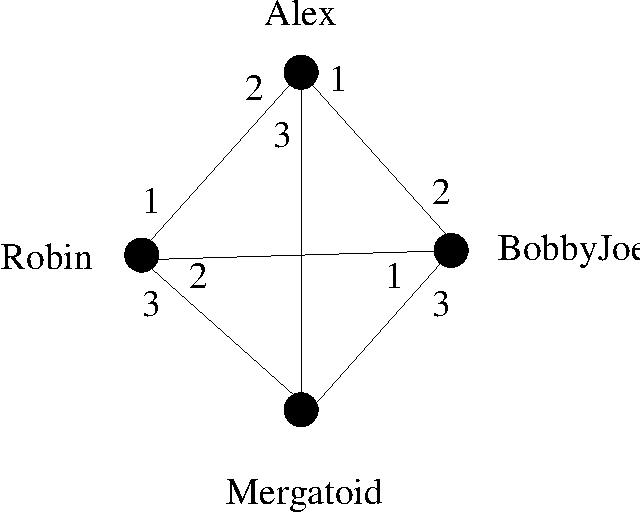
\includegraphics[height=2.3in]{figures/loveTriangle.pdf}
%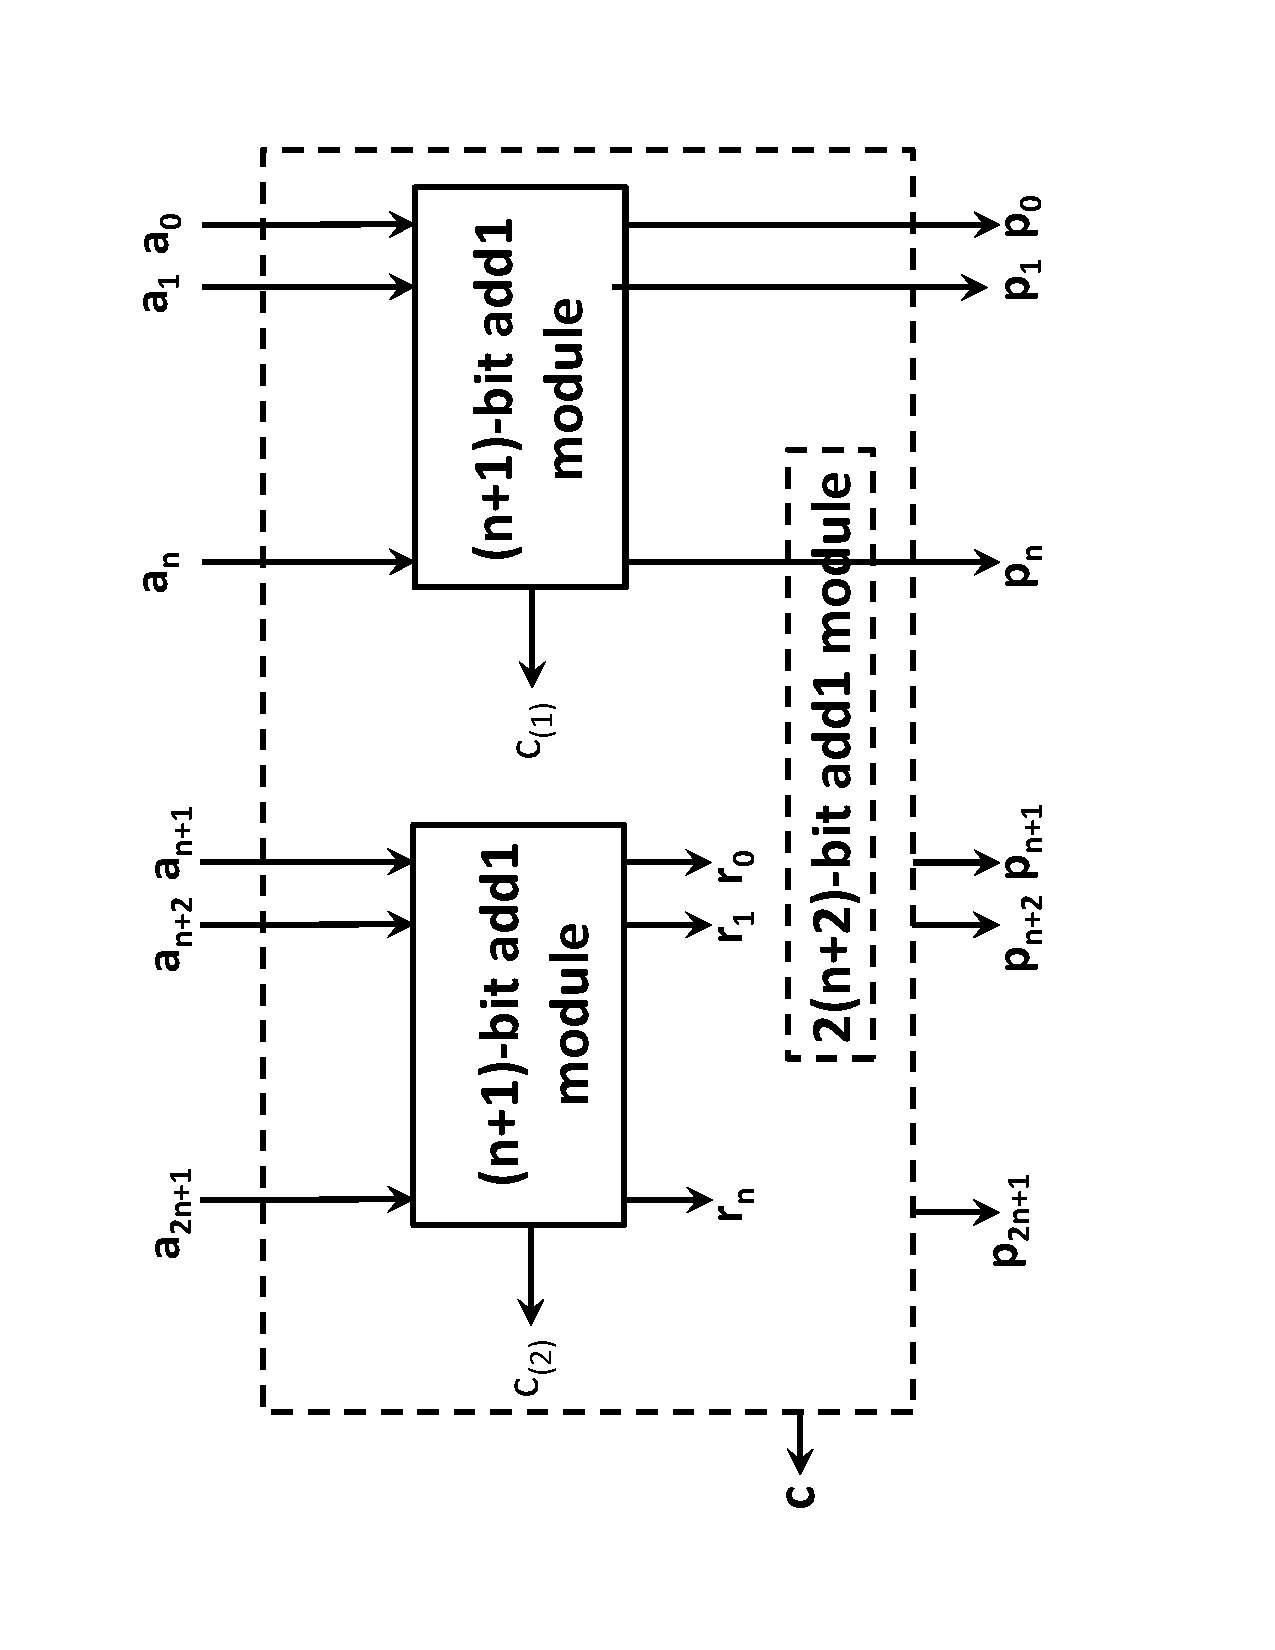
\includegraphics{latex-macros/figures/add1-circuit-diagram.pdf}
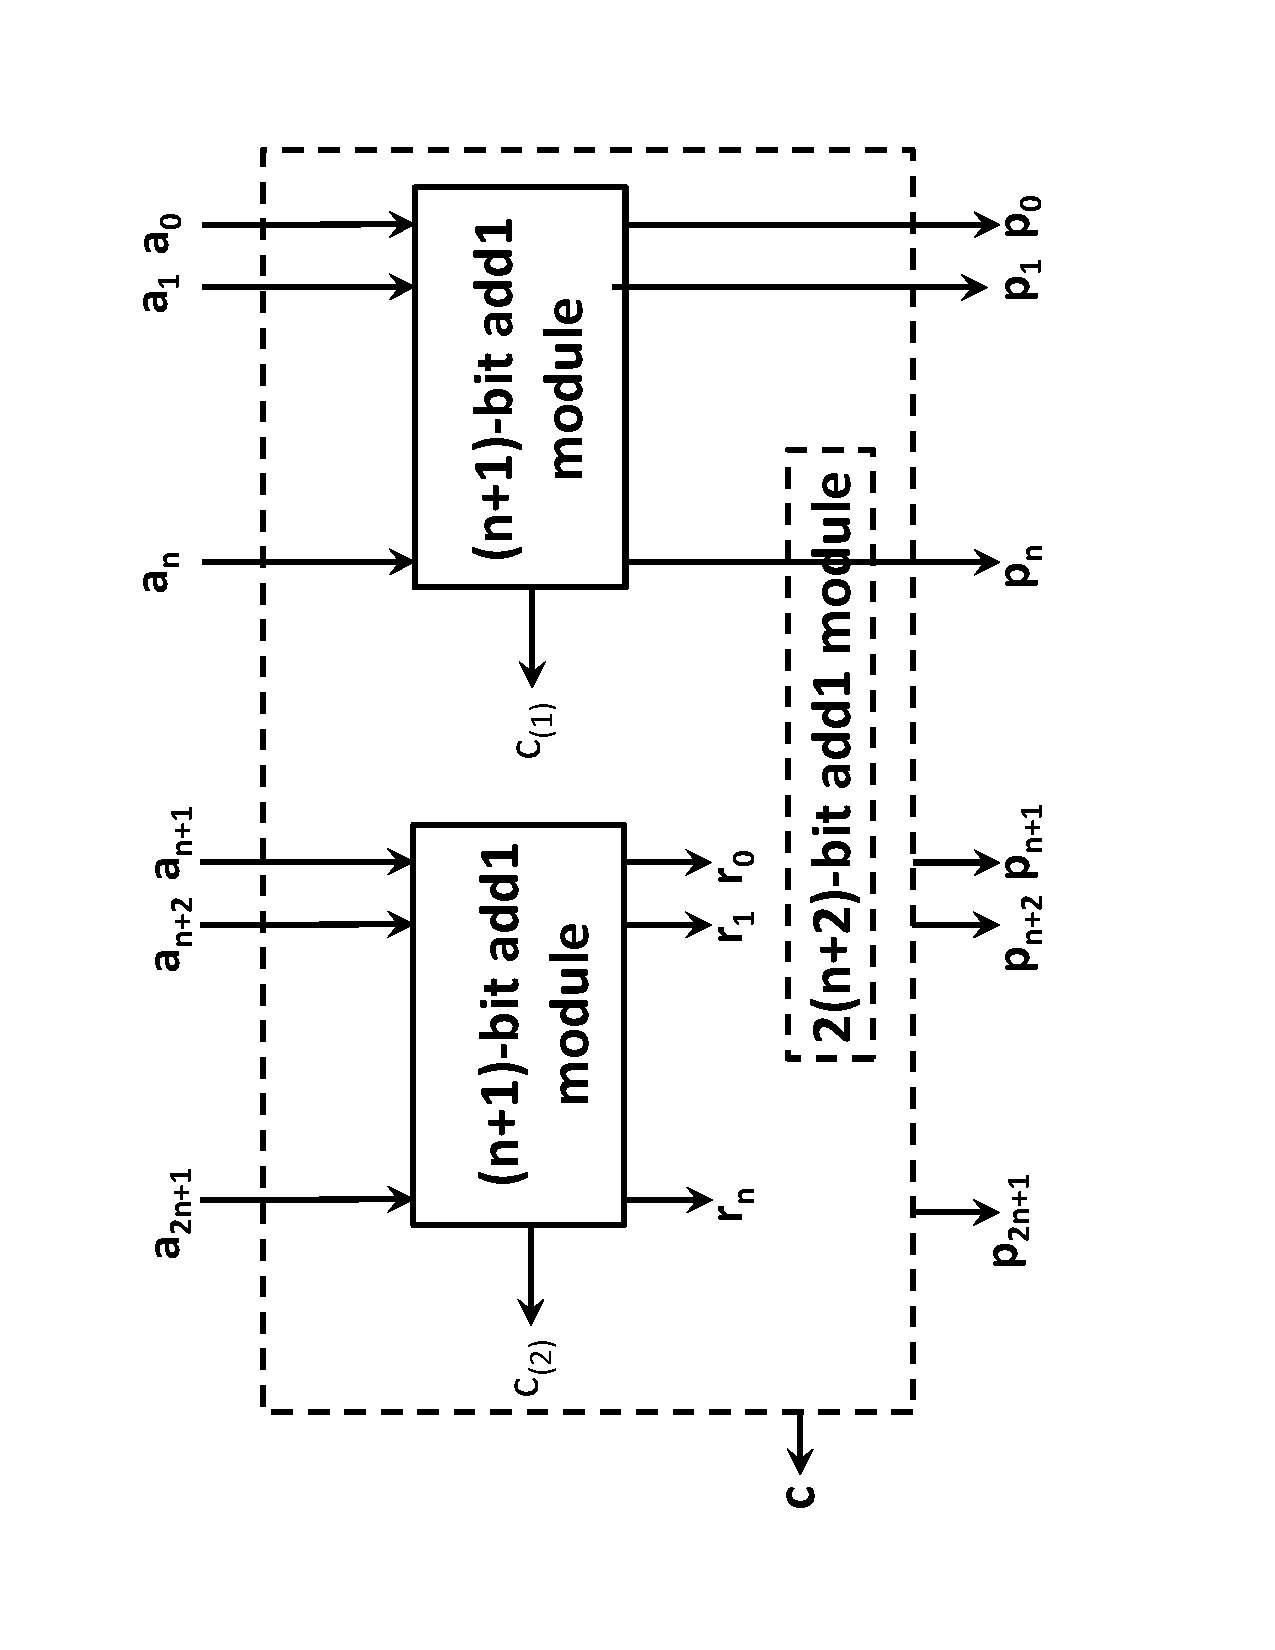
\includegraphics[height=9in]{latex-macros/figures/add1-circuit-diagram.pdf}
\caption{Structure of a Double-size Add1 Module.}
\label{fig:add1}
\end{figure}

\end{problem}

%%%%%%%%%%%%%%%%%%%%%%%%%%%%%%%%%%%%%%%%%%%%%%%%%%%%%%%%%%%%%%%%%%%%%
% Problem ends here
%%%%%%%%%%%%%%%%%%%%%%%%%%%%%%%%%%%%%%%%%%%%%%%%%%%%%%%%%%%%%%%%%%%%%
